% Chapter 3

\section{Underlying Technologies}

\subsection{Web as a platform}
One of the major decision when this project was born, was to choose the web as
the underlying platform for the application. The web provides a truly cross-platform
experience, ease of development, good security if best practices are followed.
Discite doesn't use SSL yet, which is a requirement since it do authentication, but
getting a certificate in in the process.

The are other gains by using the web as the basis of the project:
the HTTP protocol, the client-server model and the request-response provides powerful
abstractions and good isolations of components. Isolation means that each time one
makes a change on the server side, is less likely that he will damage the whole platform,
as often happens with other delivery mediums.
The request-response concept, although it provides good isolation of components,
puts the very nature of this application in danger: the goal is to have a highly interactive
application, and that is not possible with such architecture. Fortunately, the very
foundation of the web are being adapted nowadays to the new reality and new requirements.
WebRTC is such a development, one of the most fundamentally changes that web has seen since
it's birth. Another new an powerful feature is Websockets, that are not used
in this project, but were considered along with SSE, Server Sent Events, and the latter was
eventually chosen as the messaging and synchronization technology, due to it's simplicity.

The web as the platform has numerous advatages over the desktop application way
of doing things, including:
\begin{enumerate}[topsep=5pt, partopsep=0pt,itemsep=3pt,parsep=1pt]
\item[--] Good abstractions;
\item[--] Central storage of data;
\item[--] Easy sharing and collaboration;
\item[--] Hardware and OS agnostic.
\end{enumerate}
Another reason to target the web is trying to harness the collective intelligence, one of the most
appealing features that powers the web, and keeps him alive: it's massive amount of users.
% 1 page
\subsection{Ruby on Rails}
% community, activity, embraced TDD
Ruby on Rails is a MVC framework, written in the Ruby language. One of the reasons of the
choice was that it has a big community of developers. The project has been forked 8216 times,
and starred over 22 thousand times at this moment. The \href{https://github.com/rails/rails}{\texttt{rails}}
project at Github has over 2 thousands contributors.
For a developer, this means a large array of choices regarding libraries, a
wealth of tutorials and guides to follow, especially because the community is very
active in this regard: there is lots of training material, paid courses, free courses,
guides on Youtube, and usually great documentation is accompanying each library.
What makes Ruby on Rails stand out of the crowd of development frameworks is
that testing and test-driven development mantra is deeply
integrated in the core of the framework itself, and also in most of the gems
(libraries) that you can use. This makes the environment very stable (as long as you follow
the best practices too), and very easy to develop on.

Understanding the MVC pattern is key to understanding Rails. MVC divides your
application into three layers, each with a specific responsibility.
The Model layer represents your business model (such as Course, User, Person,
Post, etc.) and encapsulates the business logic that is specific to your
application. In Rails, database-backed model classes are derived from
ActiveRecord::Base. Active Record allows you to present the data from database
rows as objects and embellish these data objects with business logic methods.
Although most Rails models are backed by a database, models can also be ordinary
Ruby classes, or Ruby classes that implement a set of interfaces as provided by
the Active Model module.

The Controller layer is responsible for handling incoming HTTP requests and
providing a suitable response. Usually this means returning HTML, but Rails
controllers can also generate XML, JSON, PDFs, mobile-specific views, and more.
Controllers load and manipulate models, and render view templates in order to
generate the appropriate HTTP response. In Rails, incoming requests are routed
by Action Dispatch to an appropriate controller, and controller classes are
derived from ActionController::Base. Action Dispatch and Action Controller are
bundled together in Action Pack.

The View layer is composed of "templates" that are responsible for providing
appropriate representations of your application's resources. Templates can come
in a variety of formats, but most view templates are HTML with embedded Ruby
code (ERB files). Views are typically rendered to generate a controller
response, or to generate the body of an email. In Rails, View generation is
handled by Action View.

Active Record, Action Pack, and Action View can each be used independently
outside Rails. In addition to them, Rails also comes with Action Mailer, a
library to generate and send emails; and Active Support, a
collection of utility classes and standard library extensions that are useful
for Rails, and may also be used independently outside Rails \citep{rails_readme}.
% 3 pages
\subsection{Test-Driven Development}
Test-Driven Development is a software development methodology and strategy that
requires test to written first (the red stage), then write just enough code to
make the tests pass (the green stage), and the analyze the code written, and
change it if necessary (the refactor stage). By necessity we mean either changing
the code for performance reasons, readability, consistency with the rest of the
code base, or other reasons. The upside of this approach is that
the focus is kept on the necessary features. Also, as a refactor is done the
test suite immediately shows if those changes broke any functionality in other
parts of the application.  The downside: the test suite can get as big as actual
code that will be run. But the experience shows that it pays off in the long
term. The gains according to \citep{twelveBenefitsOfUnitTests} are:
\begin{enumerate}[topsep=5pt, partopsep=0pt,itemsep=3pt,parsep=1pt]
    \item[--] Unit tests prove that your code actually works;
    \item[--] You get a low-level regression-test suite;
    \item[--] You can improve the design without breaking it;
    \item[--] It's more fun to code with them than without;
    \item[--] They demonstrate concrete progress;
    \item[--] Unit tests are a form of sample code;
    \item[--] It forces you to plan before you code;
    \item[--] It reduces the cost of bugs;
    \item[--] It's even better than code inspections;
    \item[--] It virtually eliminates coder's block;
    \item[--] Unit tests make better designs;
    \item[--] It's faster than writing code without tests.
\end{enumerate}

There are recent concerns that TDD might induce damage on the architecture of a
application if applied improperly, and mostly due to the complexity of excessive
indirection. Some voices from the community says that coding should be less
about TDD and more about the quality of design decisions.
As usual with such confrontations, consensus is rarely reached, but the thing
that most people agree with is that test-driven development creates a
self-testing code base which is easier to improve later through refactoring, so
TDD gives you a good start point.

\subsubsection{Page Objects}
Writing plain unit tests, or feature tests comes with one drawback: the tests
can be brittle, and if tests fails, is usually hard to
tell what caused the failure. Page objects solves this sort of problem, by
concentrating all the code specific to a page inside the object: data input,
selectors, dropdowns, can be triggered from it. Usually there is a one-to-one mapping
between the pages rendered, and the page objects created. This is not a required though,
but it keeps the number of page objects manageable.
With page objects in place, if a test fails, the error thrown points to the page that caused
the error. A example of such object is presented in Listing~\ref{loginpage}, that encapsulates the
login page.
\begin{lstlisting}[language=Ruby, caption={Login Page object}, label=loginpage]
class LoginPage
  include Capybara::DSL
  include Rails.application.routes.url_helpers

  def initialize(user)
    @user = user
    visit new_user_session_path(:en)
  end

  def login
    fill_in 'email', with: @user.email
    fill_in 'password', with: @user.password
    click_on 'Sign In'
  end
end
\end{lstlisting}

The \textit{LoginPage} class isn't very useful on it's own, but is quite handy when used
in a standard Rspec test, like the one that check if the localization functionality
is working properly, as shown in Listing~\ref{localspec}. If a bug is introduced in the home page (for
example someone deletes the template that renders is), then an error is thrown in
the class \textit{LoginPage}, and this makes debugging easy.

\begin{lstlisting}[language=Ruby, caption={Localization specification}, label=localspec]
require 'spec_helper.rb'
require 'pages/profile_page'
require 'pages/login_page'

describe 'Localized application' do
  let(:user) { build(:user) }
  let(:profile) { ProfilePage.new(user) }

  xit 'should have a language switch' do
    # maybe is necessary to have a global language switch in the navigation bar
  end

  it 'should allow to set default language from profile' do
    profile.locale 'English'
    expect(user.language).to eq('en')
  end

  it 'should use the preffered language on a new session' do
    lang = :ro
    LoginPage.new(user)
    locale_file = File.open(Rails.root + "config/locales/#{lang}.yml")
    title = YAML.load(locale_file)[lang.to_s]['welcome_msg']
    profile.locale 'Romanian'
    visit '/'
    expect(page).to have_content(title)
  end
end
\end{lstlisting}

Tests that begin with \textit{xit} are disabled. In the case of the test presented in
Listing~\ref{localspec}, the code checking whether the language switch from the header is working, due
to the fact that it was never implemented, which was mainly a user experience decision.

\subsection{WebRTC}
Web Real-Time Communication (WebRTC) is a collection of standards, protocols,
and JavaScript APIs, the combination of which enables peer-to-peer audio, video,
and data sharing between browsers (peers). Instead of relying on third-party
plug-ins or proprietary software, WebRTC turns real-time communication into a
standard feature that any web application can leverage via a simple JavaScript
API, provided by the browser.

Delivering rich, high-quality, RTC applications such as audio and video
teleconferencing and peer-to-peer data exchange requires a lot of new
functionality in the browser: audio and video processing capabilities, new
application APIs, and support for half a dozen new network protocols.
Thankfully, the browser abstracts most of this complexity behind three primary
APIs:
\begin{enumerate}
    \item[--]MediaStream: acquisition of audio and video streams;
    \item[--]RTCPeerConnection: communication of audio and video data;
    \item[--]RTCDataChannel: communication of arbitrary application data.
\end{enumerate}
All it takes is a few lines of JavaScript code, and any web application can
enable a rich teleconferencing experience with peer-to-peer data transfers.
That’s the promise and the power of WebRTC. However, the listed APIs are also
just the tip of the iceberg: signaling, peer discovery, connection negotiation,
security, and entire layers of new protocols are just a few components required
to bring it all together.
Signaling is of special importance, most of the clients nowadays are behind routers, firewalls
and Network Address Translation devices, and this would make impossible direct connections with them.
Signaling is the process of coordinating communication.
In order for a WebRTC application to set up a connection, its clients need to exchange information and metadata:
\begin{enumerate}
    \item[--] Session control messages used to open, close and initialize communication;
    \item[--] Error messages;
    \item[--] Media metadata such as codecs and codec settings, bandwidth and media types;
    \item[--] Key data, used to establish secure connections;
    \item[--] Network data, such as a host's IP address and port as seen by the outside world.
\end{enumerate}

This signaling process needs a way for clients to exchange messages.
That mechanism is not implemented by the WebRTC APIs: you need to build it
yourself, or use a third-party service. The reason why a signaling
server must be used, is to avoid clients being trapped outside of the reach.
Signaling was implemented as shown in Listing~\ref{webrtc_con}. In
this case a third-party server is used, provided by nodejitsu, to simplify
deployment and management of the Discite platform.
\begin{lstlisting}[language=JavaScript, caption={WebRTC connection setup}, label=webrtc_con]
// removed code
var SIGNALING_SERVER = 'http://webrtc-signaling.nodejitsu.com:80/',
    defaultChannel = location.hash.substr(1) || location.href.replace(/\/|:|#|%|\.|\[|\]/g, '');

var channel = config.channel || defaultChannel;
var sender = Math.round(Math.random() * 999999999) + 999999999;

io.connect(SIGNALING_SERVER).emit('new-channel', {
    channel: channel,
    sender: sender
});

var socket = io.connect(SIGNALING_SERVER + channel);
socket.channel = channel;
socket.on('connect', function () {
    if (config.callback) config.callback(socket);
});

socket.send = function (message) {
    socket.emit('message', {
        sender: sender,
        data: message
    });
};
// removed code
\end{lstlisting}

The signaling protocol is actually left out of of the WebRTC specification, in order
to allow for different signaling protocol to be implemented (such as SIP, Jingle),
and the way it is used in Discite is the one specified in the JavaScript Session Establishment Protocol
(JSEP), as presented in Figure~\ref{fig:jsep}.
\begin{figure}[ht!]
    \centering
    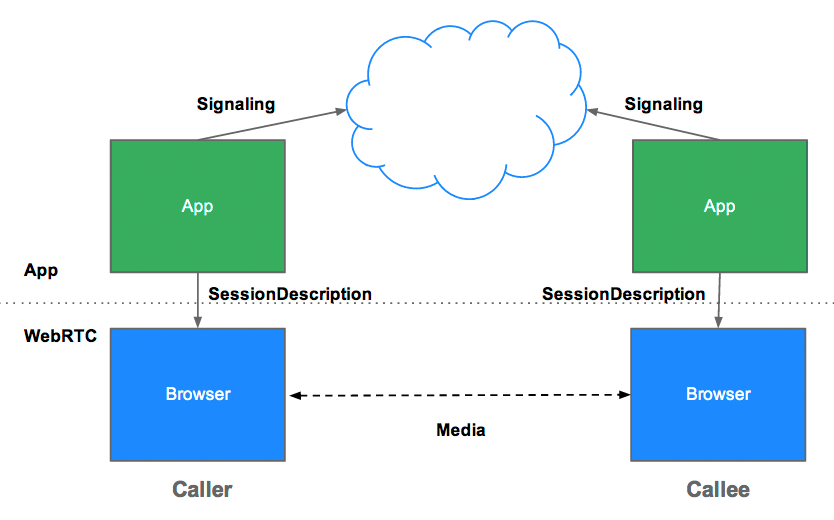
\includegraphics[height=8.5cm]{jsep}
    \caption{JSE protocol architecture}
    \label{fig:jsep}
\end{figure}
After establishing the connection, the application has to ask for streaming from specific
devices. This poses privacy and security issues, and all browsers currently require for
users to approve each time connections to the devices they want to share.
In order to get their permission, the \textit{getUserMedia} API is used, as presented in Listing~\ref{getusermedia}.
\begin{lstlisting}[language=JavaScript, caption={getUserMedia request}, label=getusermedia]
// code removed
      var video = document.createElement('video');
      video.setAttribute('autoplay', true);
      video.setAttribute('controls', true);
      videosContainer.insertBefore(video, videosContainer.firstChild);
      getUserMedia({
          video: video,
          onsuccess: function (stream) {
              config.attachStream = stream;
              video.setAttribute('muted', true);
              callback();
      }
  });
\end{lstlisting}
The application asks for both video and audio streams and by default the streaming starts muted.

Not surprisingly, the architecture and the protocols powering WebRTC also
determine its performance characteristics: connection setup latency, protocol
overhead, and delivery semantics, to name a few. In fact, unlike all other
browser communication, WebRTC transports its data over UDP. However, UDP is also
just a starting point. It takes a lot more than raw UDP to make real-time
communication in the browser a reality \citep{high_perf_browser}.

\subsection{deck.js}
\textit{deck.js} is A JavaScript library for building modern HTML presentations.
It has replaced a failed attempt to integrate \textit{ViewerJS} into the site, to make possible
to upload .pdf and .odp files, as the library doesn't support yet such a use case\citep{githubissue}.
This strategy will be evaluated in the future, but for the time being, there are several possible solutions:
\begin{enumerate}
    \item[--] upload HTML presentation directly;
    \item[--] allow uploads for .pdf's and .odp, then convert them on the server to HTML, with delayed-job and a separate worker;
    \item[--] upload .pdf's and .odp, integrate \textit{ViewerJS} in the front-end;
    \item[--] custom HTML slides editor.
\end{enumerate}
At the moment the first solution is in use, the third option has failed thus
far, there were attempts to do the second, but it complicates deployment.
The last one seems like a good option, but there wasn't enough time to explore it.

On the other hand, \textit{deck.js} is flexible enough to let advanced CSS and JavaScript authors make
highly customized decks, but also provides templates and themes for the HTML novice to build a standard
slideshow. The themes are actually not provided yet(one cannot choose what theme
his deck should use), just one of them is compressed and minified inside the assets pipeline.
\textit{deck.js} was integrated via Bower, and the necessary HTML attached to the
course rendered in a view template, as shown in Listing~\ref{deckjstemp}.
\begin{lstlisting}[language=Python, caption={deck.js template}, label=deckjstemp]
%h4 #{@course.title}, by #{@course.user.handle}, lasts #{@course.duration} hours
#presentation
  %div{"aria-role" => "navigation"}
    %a.deck-prev-link{href: "#", title: "Previous"}
    %a.deck-next-link{href: "#", title: "Next"}
  %form.goto-form{action: ".", method: "get"}
    %label{for: "goto-slide"} Go to slide:
    %input#goto-slide{list: "goto-datalist", name: "slidenum", type: "text"}/
    %datalist#goto-datalist
    %input{type: "submit", value: "Go"}/
  = render file: @slides_path
\end{lstlisting}
The \textit{deck.core} module provides all the basic functionality for creating and
moving through a deck. It applies and removes classes to indicate the state of
the deck and its slides, allowing CSS to take care of the visual representation
of each state. It also provides methods for interacting with the deck, as well
as basic key bindings for going to the next and previous slides. On top of these
basic feature, more advanced one are build, such as jumping to a specific slide, showing
the number of slide and so on. Separate extension modules provide more
functionality using the API provided by core \citep{imakewebthings}.

There are still conflicts between the CSS provided by \textit{deck.js}, the CSS from \textit{Zurb Foundation},
but most of them were solved by adding more CSS. In the pursuit to tackle this problem,
one idea that was tried was to use an iframe, that would basically make a new window
inside the browser, with it's own stylesheets and Javascript, but this wasn't feasible,
as another server was needed to stream the HTML in the iframe. This would make the application
considerably harder to maintain and deploy, so the idea was dropped.
% half a page
% move this part of the table of contents in a new page
\addtocontents{toc}{\protect\newpage}
%
\subsection{Technologies and frameworks}
In the process of building the application, a big part of the weight lifting was done by third
party libraries and frameworks. Otherwise the project would be impossible to implement by
one person. Many libraries were installed, tested, integrated, and some thrown away for
various reason.
A brief list of technologies used:
\begin{enumerate}[topsep=5pt, partopsep=0pt,itemsep=3pt,parsep=1pt]
    \item[--] Ruby - A dynamic, free programming language with a focus on
        simplicity and productivity.
        It has an elegant syntax that is natural to read and easy to write.
        \href{https://wwww.ruby-lang.org/en/}{\texttt{www.ruby-lang.org/en}}
    \item[--] \href{http://rubyonrails.org}{\texttt{Ruby on Rails}} - a MVC
        (Model-View-Controller) server-side web development framework, backed by
        the Ruby language
    \item[--] \href{http://foundation.zurb.com/}{\texttt{Zurb Foundation}} - A
        responsive front-end framework
    \item[--] \href{https://github.com/plataformatec/devise}{\texttt{Devise}} for
        authentication
    \item[--] \href{http://www.webrtc.org/}{\texttt{WebRTC}} Real-Time Communication
        implemented in browser, with a simple JavaScript API
\end{enumerate}

Ideally, the system should not require administrators and be as self-sustained as possible.
This is achievable with cloud computing, continous integration, and other such techniques.
Using Rails migration features, we try to avoid loosing data during upgrading/downgrading and
by taking advantage by another abstraction provided by Rails, namely ActiveRecord, the application
is kept independent of the RDBMS solution.

Ruby on Rails recently acquired support for streaming (with ActionController::Live),
and for server-sent events, that will be used to synchronize the presentations.
The project was started by scaffolding a few rails models (course, user), and
integrating components such as Zurb Foundation, creating header/footer, front
page, a course creation form.

These technologies were chosen because of previous experience with them, and because they
are well tested and widely deployed on production environments.
The only new and untried technology is WebRTC: is a very young project, aiming
to enable creation of rich web applications with HTML5. It's still a
\href{http://dev.w3.org/2011/webrtc/editor/webrtc.html}{\texttt{draft}} at W3C.
Nonetheless, the technology is already implemented in 2 popular browser: Google
Chrome and Mozilla Firefox.  Internet Explorer doesn't yet support it, but as
it's market share is below 10\%, we can assume that more than 80\% of web users
\citep{browserStats} will be able to use the program. As the specification will
leave the draft stage, even more supported browsers are expected.

\subsubsection{Storage systems used}
For storing data, the application uses 2 methods: the persistent data is stored
in a SQL database, and the files uploaded by the users are stored in the
file system. For the purpose of archiving the courses there might be implemented
another storage function (for video, chat), but it will not be implemented in
version 1.0 of the application. Chats will be ephemeral, they will only be kept
in users browsers as long as the course is running.

\subsection{Software Requirements Specifications}
In order for the platform to be of useful an provide value to it's end-users, a set of business
requirements have to be met such as:
\begin{enumerate}[topsep=5pt, partopsep=0pt,itemsep=3pt,parsep=1pt]
    \item[--] enables users registration
    \item[--] provides a way for users to create courses
    \item[--] enable interactive teaching process, featuring video presentation, doodling
\end{enumerate}

For users to be able to use the system safely and effectively, the system must be carefully designed
so students will find the platform familiar. To achieve that, several user requirements have
to be met:
\begin{enumerate}[topsep=5pt, partopsep=0pt,itemsep=3pt,parsep=1pt]
    \item[--] registration
    \item[--] choosing a course
    \item[--] the system should retain the user language preference
    \item[--] download materials posted by the teacher
    \item[--] chat with the teacher
    \item[--] rate the course and teacher
\end{enumerate}

Another spot were he application has received attention, is in the functional requirements department:
the application is intended to reach on as many platforms as possible (computers, tablets, phones), and and
as many users as possible. Phones with a certain screen resolution are not supported, unfortunately, as it
would cripple the whole experience for other users, but recent smartphones
should do the job. This means that the application should:
\begin{enumerate}[topsep=5pt, partopsep=0pt,itemsep=3pt,parsep=1pt]
    \item[--] be internationalized
    \item[--] support file uploads via AJAX
    \item[--] the interface should be responsive (800x600 up to 4k resolution)
    \item[--] WebRTC video/audio streams
\end{enumerate}

To avoid frustration while using the site, some performance and quality-of-service requirements
must reached:
\begin{enumerate}[topsep=5pt, partopsep=0pt,itemsep=3pt,parsep=1pt]
    \item[--] it should work without issues for at least 4 hours
    \item[--] each page should have tests
    \item[--] each module should be tested with rspec
    \item[--] the application should be behavior-driven tested with capybara + RSpec
    \item[--] supporting at least up to 200 users simultaneously (apprx. 10-20 courses at a time)
    \item[--] deployment by a skilled administrator should take less than 30 min.
\end{enumerate}

